\section{Obstruction of Myopic Error-Monotone Control and Rational KKT Certificate}\label{sec:obstruction}

\subsection{Variational Inequality and Normal-Cone Lock-Up of Myopic Projections}
In standard safety-critical navigation \cite{ames2017cbf,reis2021}, each robot uses the proportional goal-attraction nominal law $\bu_i^{\mathrm{nom}}=-k_g\be_i=-k_g(\bp_i-\bg_i)$ ($k_g>0$), yielding the filtered input $\bu_G=\Pi_{\mathcal K_0(\bp)}(-k_g\be)$. By the variational inequality of Euclidean projection onto the closed convex set $\mathcal K_0(\bp)$,
\begin{equation}
 (\bu_G+k_g\be)^{\top}(\boldsymbol v-\bu_G)\ge 0,\qquad\forall\boldsymbol v\in\mathcal K_0(\bp).
 \label{eq:vi-proj}
\end{equation}
Substituting the always-safe zero velocity $\boldsymbol v=\boldsymbol 0\in\mathcal K_0(\bp)$ into \eqref{eq:vi-proj} yields
\begin{equation}
 \dot W(\bp)=\be^{\top}\bu_G\le -\frac{1}{k_g}\norm{\bu_G}_2^2\le 0.
 \label{eq:W-descent}
\end{equation}
Equation~\eqref{eq:W-descent} shows that whenever $\boldsymbol 0\in\mathcal K_0(\bp)$, any proportional-attraction safety filter enforces monotone nonincreasing $W(\bp(t))$. However, at a non-target configuration ($\be\ne\boldsymbol 0$), if $-k_g\be$ falls into the normal cone $N_{\mathcal K_0(\bp)}(\boldsymbol 0)=\{\boldsymbol w\in\mathbb R^{2N}:\boldsymbol w^{\top}\boldsymbol v\le 0,\ \forall\boldsymbol v\in\mathcal K_0(\bp)\}$ \cite{rockafellar1970}, no nonzero safe velocity can decrease $W$ to first order, and the unique global optimum of the safety QP collapses to $\bu_G=\boldsymbol 0$.

\subsection{Seven-Robot Strict Non-Target Local Minimum Theorem and Energy Barrier}\label{subsec:seven-kkt}
Deadlocks in CBF filters are often treated as unstable saddle points escapable via small perturbations or negative curvature \cite{reis2021,tan2024equilibria}. To rigorously falsify the universality of this assumption when all robots are mobile, consider the seven-robot planar symmetric double-triangle configuration $\bar\bp\in\mathbb R^{14}$ shown in Fig.~\ref{fig:seven-geom}(a) ($\ds=1\ \mathrm m,U=1/2\ \mathrm{m/s}$, columns correspond to robots $1,\dots,7$):
\begin{equation}
 \bar\bp^{\top}=\begin{bmatrix}
 -1 & -1/2 & -1/2 & 0 & 1/2 & 1/2 & 1\\
 0 & \sqrt{3}/2 & -\sqrt{3}/2 & 0 & \sqrt{3}/2 & -\sqrt{3}/2 & 0
 \end{bmatrix}.
 \label{eq:seven-config}
\end{equation}
At $\bar\bp$, all $7$ robots are mobile and form $12$ active contact edges at $d_{ij}=1\ \mathrm m$: $\mathcal E_c=\{12,13,14,24,25,34,36,45,46,47,57,67\}$. Outer robots $1,2,3,5,6$ start at their respective goals ($\bg_i=\bar\bp_i,\be_i=\boldsymbol 0$), whereas center robot $4$ at $(0,0)$ and rightmost robot $7$ at $(1,0)$ must exchange positions ($\bg_4=\bar\bp_7,\bg_7=\bar\bp_4$).

\begin{figure*}[htbp]
 \centering
 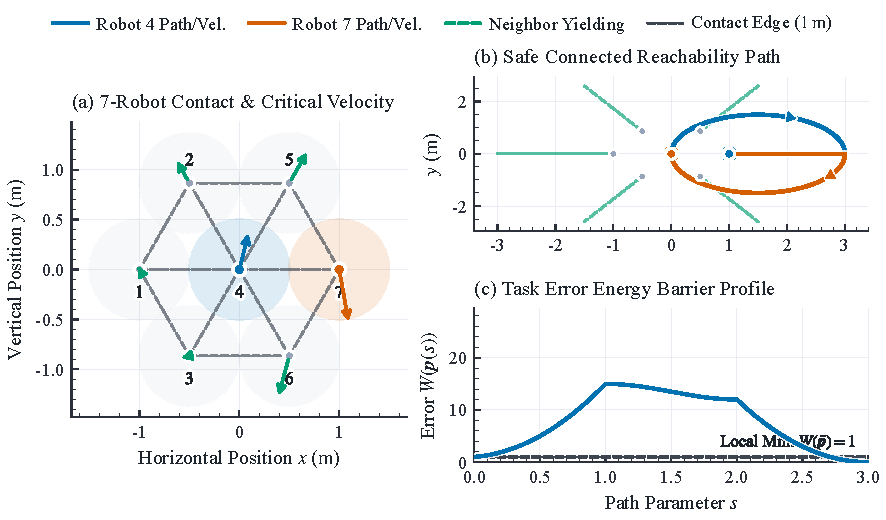
\includegraphics[width=\textwidth]{figures_en/fig1_seven_geometry.pdf}
 \caption{Seven-robot strict non-target local minimum configuration and analytical safe connected reachability witness. (a) Double-triangle contact configuration \eqref{eq:seven-config}, $12$ initial contact edges, and optimal critical-cone velocity witness vectors \eqref{eq:certificate-primal}; (b) analytical 3-stage reachability path (uniform expansion by $3$, opposite semicircular swap of robots $4$ and $7$, and uniform contraction); (c) task error profile $W(\bp(s))$ along the witness path, illustrating the mandatory energy barrier above $W(\bar\bp)=1$.}
 \label{fig:seven-geom}
\end{figure*}

\begin{theorem}[Exact Rational Certificate of Strict Local Minimum and Energy Barrier]\label{thm:seven-kkt}
For the seven-robot position swap task \eqref{eq:seven-config} with $\ds=1\ \mathrm m,\lr=5/2,R_c=10\ \mathrm m$:
\begin{enumerate}
 \item \textbf{First-order stationarity and second-order strict positive definiteness on the critical cone:} At $\bar\bp$, $W(\bar\bp)=1$, $\lambda_2(\bL(\bar\bp))>5/2$, and $\nabla W(\bar\bp)=\frac12\nabla h_{47}^{\mathrm{col}}(\bar\bp)$, so $\bu_G=\boldsymbol 0$ is the unique optimum of \eqref{eq:central-proj}. Over the full critical cone $\mathcal C=\{\boldsymbol v\in\mathbb R^{14}:\bar\bp_{ij}^{\top}(\boldsymbol v_i-\boldsymbol v_j)\ge 0\ (\forall\{i,j\}\in\mathcal E_c),\ v_{4x}=v_{7x}\}$, the Lagrangian Hessian $\boldsymbol H_L=\I_{14}-(\boldsymbol b_{47}\boldsymbol b_{47}^{\top})\otimes\I_2$ satisfies the exact rational bounds:
 \begin{equation}
 \begin{split}
  \min_{\boldsymbol v\in\mathcal C,\ v_{4y}-v_{7y}=1}\norm{\boldsymbol v}_2^2&=\frac{515}{496}>1,\\
  \boldsymbol v^{\top}\boldsymbol H_L\boldsymbol v&\ge\frac{19}{515}\norm{\boldsymbol v}_2^2>0\quad(\forall\boldsymbol v\in\mathcal C\setminus\{\boldsymbol 0\}).
 \end{split}\label{eq:critical-hessian}
 \end{equation}
 \item \textbf{Finite-radius spherical energy barrier and strictly interior open-ball trap:} For every collision-free perturbation $0<\norm{\boldsymbol\delta}_2\le\frac1{200}$ satisfying $d_{ij}(\bar\bp+\boldsymbol\delta)\ge 1$ ($\forall i<j$),
 \begin{equation}
  W(\bar\bp+\boldsymbol\delta)-W(\bar\bp)\ge\frac{1}{100}\norm{\boldsymbol\delta}_2^2>0.
  \label{eq:finite-barrier}
 \end{equation}
 Moreover, for the strictly interior perturbed task $\bp_0=(1+10^{-8})\bar\bp,\bg_\tau=(1+10^{-6})\bg$, every continuous safe trajectory starting in the open ball $B_\rho(\bp_0)\subset\operatorname{int}(\mathcal S)$ of radius $\rho=\frac{1}{4\times 10^8}$ with $\dot W_\tau\le 0$ is permanently trapped inside the sphere $\norm{\bp-\bar\bp}_2=\frac1{200}$ ($W_\tau(\bar\bp+\boldsymbol\delta)-W_\tau(\bar\bp)\ge\frac{19}{8\times 10^7}>W_\tau(\bp)-W_\tau(\bar\bp)$) and cannot reach the exterior goal $\bg_\tau$.
 \item \textbf{Global collision-free and spectrally connected reachability:} There exists an explicit piecewise smooth path $\bp(s)$ ($s\in[0,3]$) connecting the initial and goal configurations such that $d_{ij}(s)\ge 1\ \mathrm m$ and $\lambda_2(\bL(\bp(s)))\ge\frac{1792}{625}=2.8672>\frac52$ for all $s\in[0,3]$.
\end{enumerate}
\end{theorem}
\begin{proof}
(1) At $\bar\bp$, $\be_4=(-1,0)^{\top},\be_7=(1,0)^{\top}$, and $\be_i=\boldsymbol 0$ otherwise, while $\nabla_{\bp_4}h_{47}^{\mathrm{col}}(\bar\bp)=(-2,0)^{\top}$ and $\nabla_{\bp_7}h_{47}^{\mathrm{col}}(\bar\bp)=(2,0)^{\top}$; thus multiplier $\lambda_{47}=1/2$ (and $0$ on all other edges) satisfies $\nabla W(\bar\bp)-\frac12\nabla h_{47}^{\mathrm{col}}(\bar\bp)=\boldsymbol 0$. For $\boldsymbol v\in\mathcal C$, $\boldsymbol v^{\top}\boldsymbol H_L\boldsymbol v=\norm{\boldsymbol v}_2^2-|v_{4y}-v_{7y}|^2$. Scaling coordinates as $\boldsymbol v_i=(z_{ix},\sqrt{3}z_{iy})^{\top}$ stacked into $\boldsymbol z\in\mathbb R^{14}$ with $Q_c=\diag(1,3,\dots,1,3)$ gives $\norm{\boldsymbol v}_2^2=\boldsymbol z^{\top}Q_c\boldsymbol z$. Define rational matrices $(G_c\boldsymbol z)_{ij}=\bar p_{ij,x}(z_{ix}-z_{jx})+\sqrt{3}\bar p_{ij,y}(z_{iy}-z_{jy})$ and $E_c\boldsymbol z=[z_{4x}-z_{7x},\,z_{4y}-z_{7y}]^{\top}$. For the convex QP $\min\boldsymbol z^{\top}Q_c\boldsymbol z\ \text{s.t.}\ G_c\boldsymbol z\ge\boldsymbol 0,\,E_c\boldsymbol z=(0,1)^{\top}$, the exact rational primal witness $Z_*\in\mathbb Q^{7\times 2}$ and dual multipliers $(\boldsymbol\mu,\boldsymbol\nu)$ are:
\begin{equation}
\begin{split}
 Z_*^{\top}&=\frac{1}{496}{\setlength{\arraycolsep}{2.5pt}\begin{bmatrix}
 -15 & -132 & -105 & 90 & 177 & -105 & 90\\
 15 & 132 & -15 & 206 & 177 & -225 & -290
 \end{bmatrix}},\\
 \mu_{13}&=\tfrac{15}{248},\ \mu_{24}=\tfrac{33}{62},\ \mu_{36}=\tfrac{15}{62},\ \mu_{45}=\tfrac{177}{248},\ \mu_{67}=\tfrac{225}{248},\\
 \boldsymbol\nu&=\big[\tfrac{135}{496},\,\tfrac{1545}{496}\big]^{\top},
\end{split}\label{eq:certificate-primal}
\end{equation}
with all other $\mu_{ij}=0$. Exact rational arithmetic verifies primal feasibility $G_c\boldsymbol z_*\ge\boldsymbol 0,E_c\boldsymbol z_*=(0,1)^{\top}$, complementary slackness $\boldsymbol\mu^{\top}G_c\boldsymbol z_*=0$, and stationarity $Q_c\boldsymbol z_*=G_c^{\top}\boldsymbol\mu+E_c^{\top}\boldsymbol\nu$, with optimal objective $\boldsymbol z_*^{\top}Q_c\boldsymbol z_*=\frac{1545}{496}$. Dividing by the vertical scaling factor $3$ yields $\min_{\boldsymbol v\in\mathcal C,v_{4y}-v_{7y}=1}\norm{\boldsymbol v}_2^2=\frac{515}{496}>1$ and $\boldsymbol v^{\top}\boldsymbol H_L\boldsymbol v\ge(1-\frac{496}{515})\norm{\boldsymbol v}_2^2=\frac{19}{515}\norm{\boldsymbol v}_2^2$.

(2) Let $0<R:=\norm{\boldsymbol\delta}_2\le\frac1{200}$ satisfy $\norm{\bar\bp_{ij}+\boldsymbol\delta_i-\boldsymbol\delta_j}_2^2\ge 1$ ($\forall\{i,j\}\in\mathcal E_c$). With $z=\delta_{4x}-\delta_{7x}$ and $t=\delta_{4y}-\delta_{7y}$, we have $W(\bar\bp+\boldsymbol\delta)-W(\bar\bp)=\frac12 R^2-z$. If $z\le 0$, \eqref{eq:finite-barrier} holds trivially; suppose $z>0$. Each contact edge gives $\bar\bp_{ij}^{\top}(\boldsymbol\delta_i-\boldsymbol\delta_j)\ge -\frac12\norm{\boldsymbol\delta_i-\boldsymbol\delta_j}_2^2\ge -R^2$. Taking the inner product of $Q_c\boldsymbol z_*=G_c^{\top}\boldsymbol\mu+E_c^{\top}\boldsymbol\nu$ with the scaled perturbation $\tilde{\boldsymbol\delta}$, using $\sum\mu_{ij}=\frac{609}{248}=:S$, $c=\frac{1545}{496}$, and the Cauchy--Schwarz inequality gives $\frac{c}{\sqrt{3}}|t|\le\sqrt{c}R+SR^2\implies t^2\le\frac{496}{515}R^2(1+\frac32 R)^2$. Moreover, $(-1+z)^2+t^2\ge 1\implies 2z\le z^2+t^2$ and $z\le 2R^2$, whence
\begin{equation}
\begin{split}
 W(\bar\bp+\boldsymbol\delta)-W(\bar\bp)&=\frac12 R^2-z\\
 &\ge\frac{R^2}{2}\left[1-\frac{496}{515}\Big(1+\frac32 R\Big)^2-4R^2\right]\\
 &\ge\frac{1}{100}R^2,\qquad\forall R\in\Big(0,\frac1{200}\Big].
\end{split}
\end{equation}
The strictly interior trap on $B_\rho(\bp_0)$ follows from $W_\tau(\bar\bp+\boldsymbol\delta)-W_\tau(\bar\bp)\ge\frac{r^2}{100}-\frac52\tau r=\frac{19}{8\times 10^7}$ on $\norm{\boldsymbol\delta}_2=r=\frac1{200}$.

(3) Along the 3-stage path in Fig.~\ref{fig:seven-geom}(b) (uniform expansion to $3\bar\bp$, opposite semicircular swap of robots $4$ and $7$ around $(3/2,0)$ with radius $3/2$, and uniform contraction to $\bg$), all pairwise distances satisfy $d_{ij}(s)\ge 1$ and $\max_{i<j}d_{ij}(s)\le 6$, so $w_{ij}(s)\ge(1-36/100)^2=256/625$ and $\lambda_2(\bL(\bp(s)))\ge 7\times\frac{256}{625}=\frac{1792}{625}>\frac52$.
\end{proof}

\begin{remark}[Two Necessary and Sufficient Physical Conditions for Deadlock Resolution]\label{rem:two-conditions}
The exact rational witness \eqref{eq:certificate-primal} establishes two fundamental physical conditions required to unlock dense interior swaps:
\begin{enumerate}
 \item \textbf{Lateral symmetry-breaking nominal drive from swapping robots:} In \eqref{eq:certificate-primal}, robots $4$ and $7$ must generate opposite transverse velocity components $z_{4y}=+\frac{206}{496}>0$ and $z_{7y}=-\frac{290}{496}<0$ perpendicular to $\be_4,\be_7$. Purely radial attraction keeps the system inside the collinear deadlock subspace $v_{4y}-v_{7y}=0$.
 \item \textbf{Cooperative yielding of outer stationary neighbors via dynamic quota transfer:} As robots $4$ and $7$ separate transversely, the five outer target-holding neighbors ($\be_j=\boldsymbol 0$) must simultaneously execute nonzero outward yielding velocities (e.g., $(Z_*)_{2,:}=\frac1{496}[-132,132]$, $(Z_*)_{5,:}=\frac1{496}[177,177]$), transmitted mechanically through strictly positive contact shadow prices $\mu_{24},\mu_{45},\mu_{67}>0$. Under static equal quota splitting ($s_{ia}\equiv 0$), stationary neighbors remain frozen at $\bu_j=\boldsymbol 0$ and truncate the transverse separation of robots $4$ and $7$ to zero.
\end{enumerate}
\end{remark}
